\documentclass{article}
\usepackage[utf8]{inputenc}
\usepackage[a4paper, total={7in, 10in}]{geometry}
\usepackage{hyperref}
\usepackage{mathtools}
\hypersetup{
    colorlinks=true,
    linkcolor=blue,
    filecolor=magenta,      
    urlcolor=black,
}

\title{Data Mining Final Report }
\author{Kadir Karayakalı , Berkcan Erguncu, Mandana Zooyousefin  }
\date{January 2021}

\usepackage{natbib}
\usepackage{graphicx}


\begin{document}

\maketitle

\section{Introduction}

To manually classify a music sample or song, one needs to listen to the song and select the genre. This process takes a lot of time one should also know about different types of music. Being able to instantly classify songs in any given playlist or library by genre is an important functionality for any music streaming or purchasing service. Our system takes the piece of music, then converts it into numerical values with some operations, then determines the possible genre by comparing it with our data. Python has a library called "Librosa" to convert audio files to numeric data, from which we can create the numerical data we need.



\section{ Description of Data Set}


GTZAN genre collection was used as our dataset. The dataset consists of 1000 audio tracks each 30 seconds long. It contains 10 genres, each represented by 100 tracks. Tracks are wav(Waveform Audio File) formats. This tracks will transform digital datas. \newline
Source: \underline{\url{http://marsyas.info/downloads/datasets.html}} \newline
\newline
Our digital data columns and descriptions;\newline
\textbf{Zero Crossing Rate: } The zero crossing rate is the rate of sign-changes along a signal, i.e., the rate at which the signal changes from positive to negative or back. \newline
\textbf{Spectral Centroid: } It indicates where the ”centre of mass” for a sound is located and is calculated as the weighted mean of the frequencies present in the sound.\newline
\textbf{Spectral Rolloff:} It is a measure of the shape of the signal. It represents the frequency below which a specified percentage of the total spectral energy, e.g. 85\%, lies. \newline
\textbf{Spectral Bandwidth: } It is the wavelength interval in which a radiated spectral quantity is not less than half its maximum value.\newline
\textbf{Mel-Frequency Cepstral Coefficients: } The Mel frequency cepstral coefficients (MFCCs) of a signal are a small set of features (usually about 10–20) which concisely describe the overall shape of a spectral envelope.\newline
\textbf{Chroma Frequencies:} Chroma features are an interesting and powerful representation for music audio in which the entire spectrum is projected onto 12 bins representing the 12 distinct semitones (or chroma) of the musical octave.One of the main features of Chroma features is that they are harmonic and melodic, while being robust against changes in timbre and instrumentation.\newline

\section{ Data Preprocess}

\subsection{Data Tranformation }
This tracks is transformed to digital data by using Python Librosa. Librosa is a Python module to analyze audio signals in general but geared more towards music. 
-Audio files were read with librosa library and converted into objects
-Required properties were transferred to variables with librosa library. The properties are generally written to the csv file in averages, as they represent a graphic and have a different value every second. \

\subsection{PCA : Principal Component Analysis }

The principal components of a collection of points in a real p-space that are a sequence of p direction vectors, where the i vector is the direction of a line that best fits the data while being orthogonal to the first i-1 vectors. Here, a best-fitting line is defined as one that minimizes the average squared distance from the points to the line. These directions constitute an orthonormal basis in which different individual dimensions of the data are linearly uncorrelated. Principal component analysis (PCA) is the process of computing the principal components and using them to perform a change of basis on the data, sometimes using only the first few principal components and ignoring the rest.\newline

When we run the PCA function in the Sci-kit library with the 95\% parameter, 15 valued components were found. The graph with the variant curve is as follows.


\begin{center}
    \vspace{1em}
        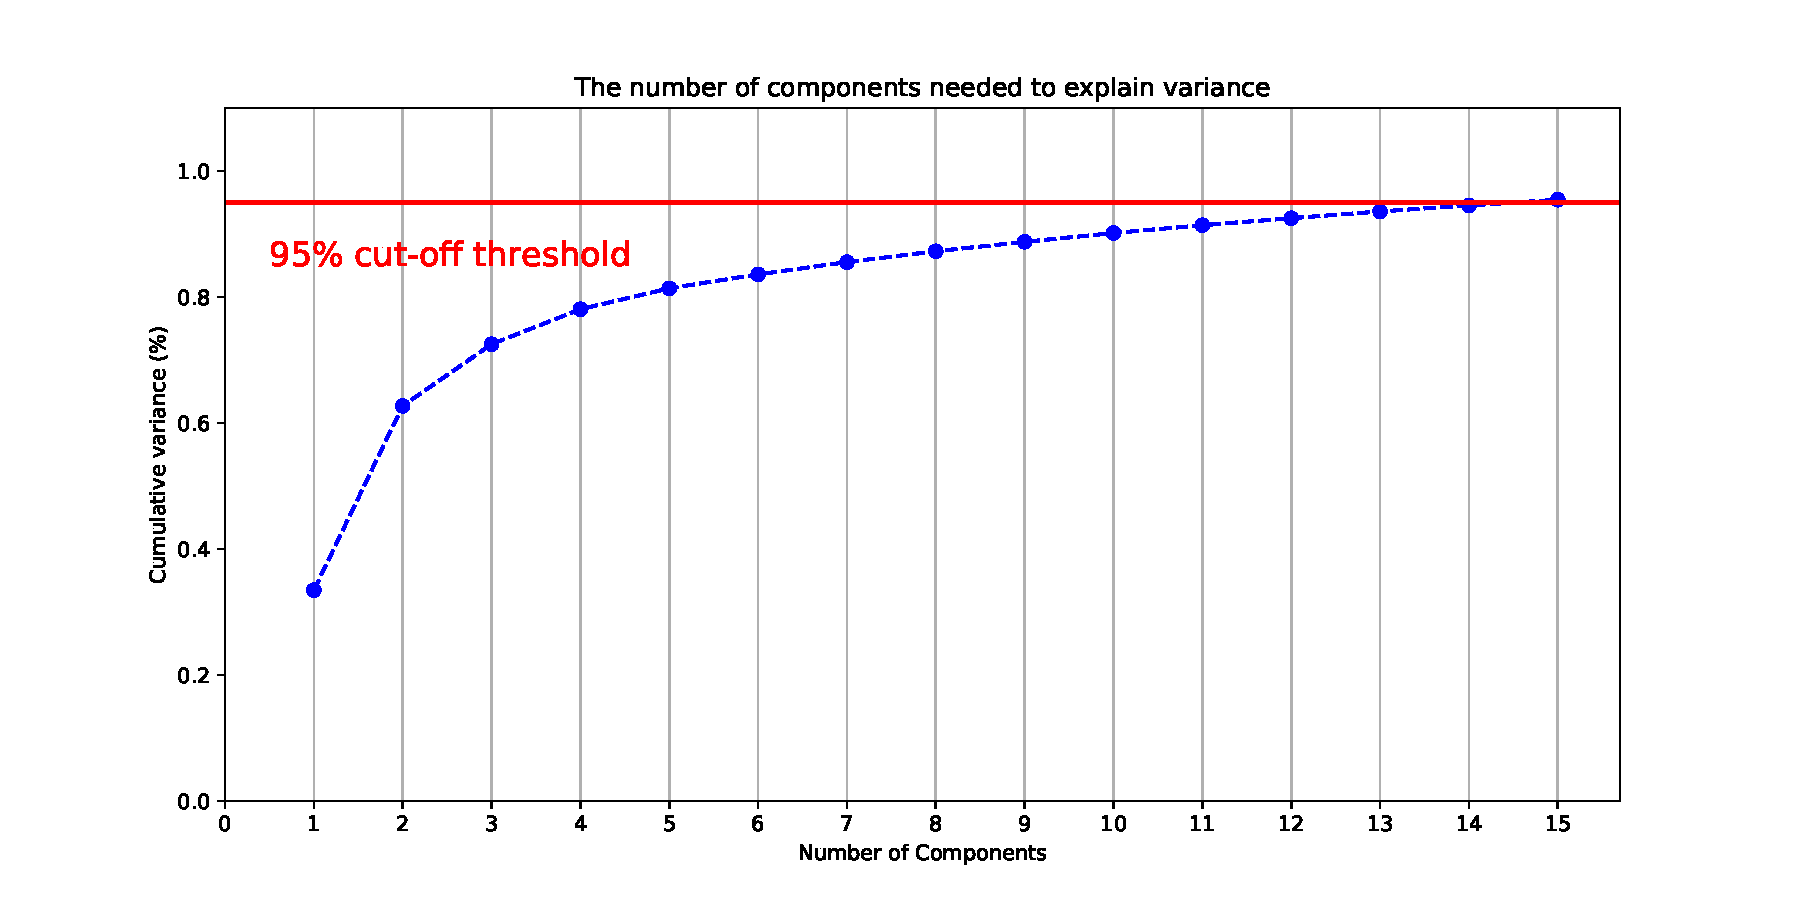
\includegraphics[scale=0.55]{graphs/Pca_Test.pdf}
    \vspace{1em}
\end{center}

\section{ Machine Learning Problem And Analysis}

Test data has 10 different music genre like hip hop, rock, pop, jazz, metal, blues, classical, disco, reggae, country. Our goal is predict genres of new musics for some application. Determining music genres is to use classification model so machine learning category is “Classification”. For that purpose three different machine learning algorithms and also with bagging algorithm was used. These algorithms are K-Nearest Neighbors, Support Vector Machine, Neural Network. 10-fold cross-validation used for testing these algorithms. These algorithms train with raw data and data which applied PCA. \newline

\subsection{ K-NN Algorithm}

k-NN is a type of instance-based learning, or lazy learning, where the function is only approximated locally and all computation is deferred until function evaluation. Since this algorithm relies on distance for classification, if the features represent different physical units or come in vastly different scales then normalizing the training data can improve its accuracy dramatically.\newline

\begin{center}
    \vspace{1em}
        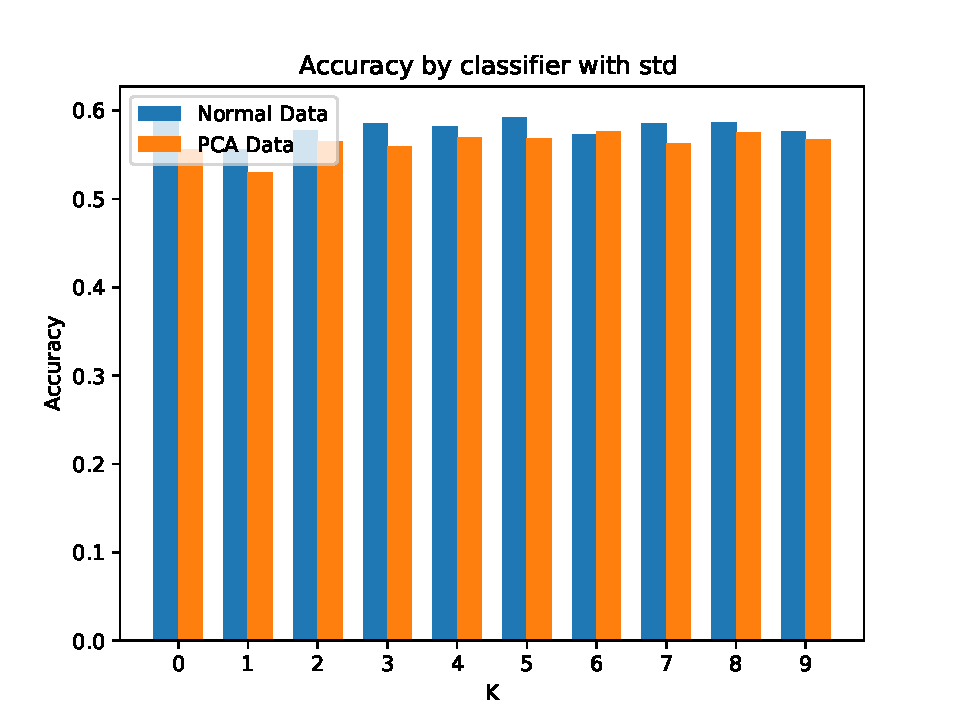
\includegraphics[scale=0.80]{graphs/KNN.pdf}
    \vspace{1em}
\end{center}

When tested with a number of neighbors from 1 to 10, it was observed that the number of neighbors was not a major factor for accuracy. For this reason, it was decided to accept the number of neighbors as 5. It has been observed that the train model applied with PCA gives lower performance compared to the original data. The graphic regarding the results is as above.


\subsection{ SVM (Support Vector Machine)}

More formally, a support-vector machine constructs a hyperplane or set of hyperplanes in a high- or infinite-dimensional space, which can be used for classification, regression, or other tasks like outliers detection. Intuitively, a good separation is achieved by the hyperplane that has the largest distance to the nearest training-data point of any class (so-called functional margin), since in general the larger the margin, the lower the generalization error of the classifier. 

\begin{center}
    \vspace{1em}
        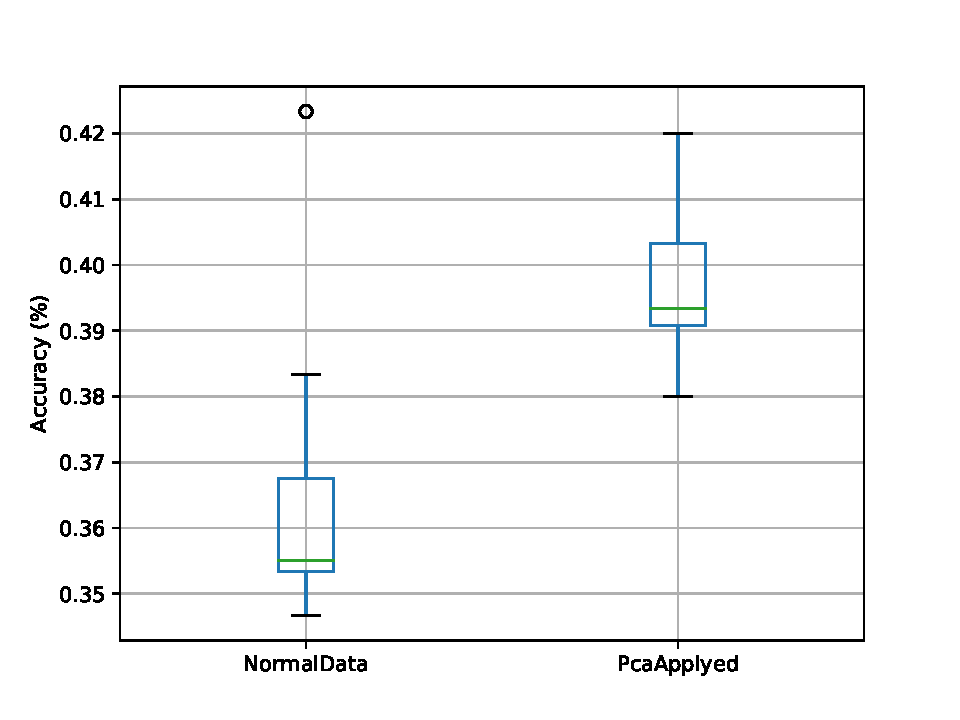
\includegraphics[scale=0.75]{graphs/SVM.pdf}
    \vspace{1em}
\end{center}

Original data and PCA applied data were trained on SVM model. Boxplot was used for the result observation. The PCA applied data showed better accuracy, but overall, the accuracy did not exceed 50\%. The graphic regarding the results is as above.


\subsection{ Neural Network (MLP)}

A neural network is a network or circuit of neurons, or in a modern sense, an artificial neural network, composed of artificial neurons or nodes. Thus a neural network is either a biological neural network, made up of real biological neurons, or an artificial neural network, for solving artificial intelligence (AI) problems. The connections of the biological neuron are modeled as weights. A positive weight reflects an excitatory connection, while negative values mean inhibitory connections. All inputs are modified by a weight and summed. This activity is referred to as a linear combination. Finally, an activation function controls the amplitude of the output. For example, an acceptable range of output is usually between 0 and 1, or it could be -1 and 1.

\begin{center}
    \vspace{1em}
        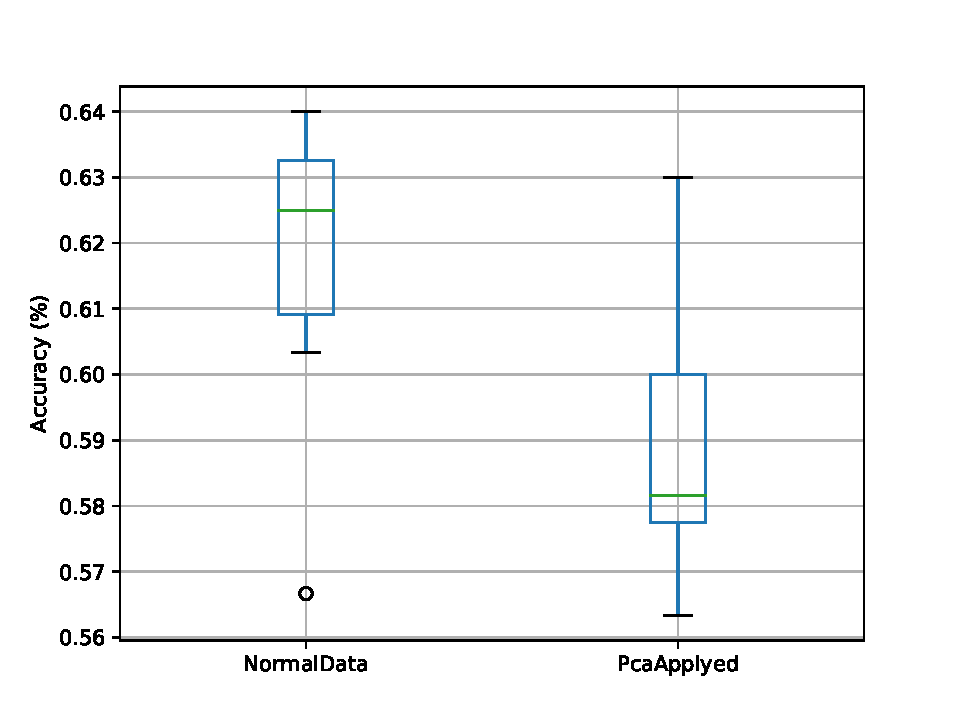
\includegraphics[scale=0.75]{graphs/MLP.pdf}
    \vspace{1em}
\end{center}

The original data and the PCA applied data were trained on the MLP model. Boxplot was used for the result observation. PCA-treated data showed worse consistency. It showed better accuracy compared to KNN and SVM.The graphic regarding the results is as above.



\subsection{ Bagging }

Bootstrap aggregating, also called bagging (from bootstrap aggregating), is a machine learning ensemble meta-algorithm designed to improve the stability and accuracy of machine learning algorithms used in statistical classification and regression. It also reduces variance and helps to avoid overfitting. Although it is usually applied to decision tree methods, it can be used with any type of method. Bagging is a special case of the model averaging approach.

\begin{center}
    \vspace{1em}
        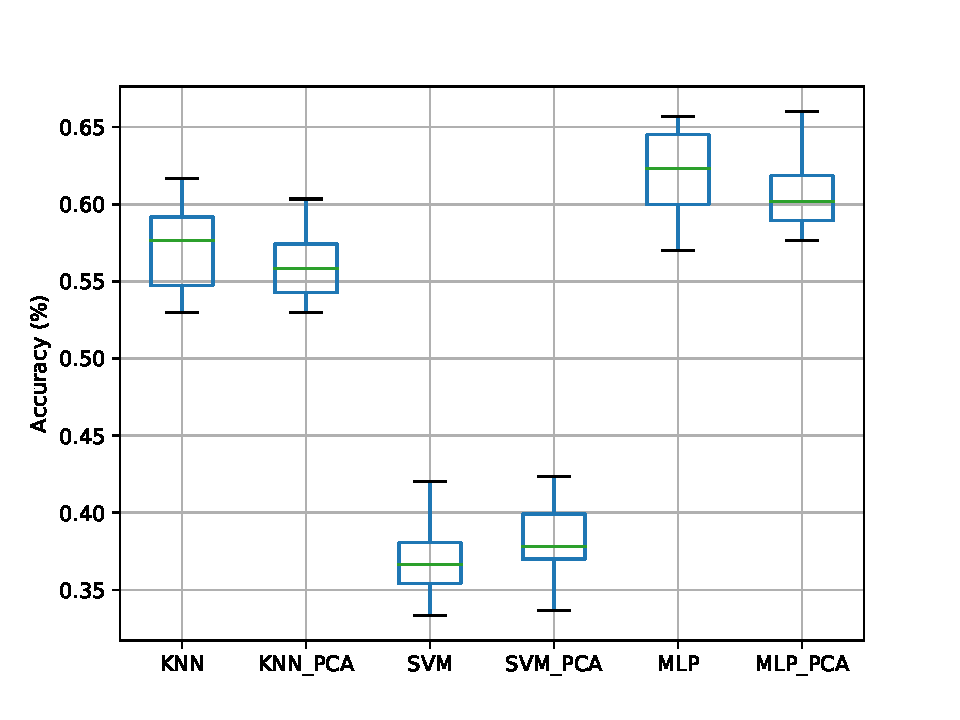
\includegraphics[scale=0.75]{graphs/BaggingClassifier.pdf}
    \vspace{1em}
\end{center}

An improvement was expected in all 3 methods used after bagging was applied, but as seen from the results, no visible improvement was observed. The results obtained are almost the same as the results without bagging. It is concluded that bagging is a costly process that does not work for this data.The graphic regarding the results is as above.


\section{ Conclusion}

In conclusion, to get better results for this project, 3 different classifiers have been tried as KNN, Support Vector Machine,  Neural Network and with Bagging  with Python. 

\begin{center}
    \vspace{1em}
        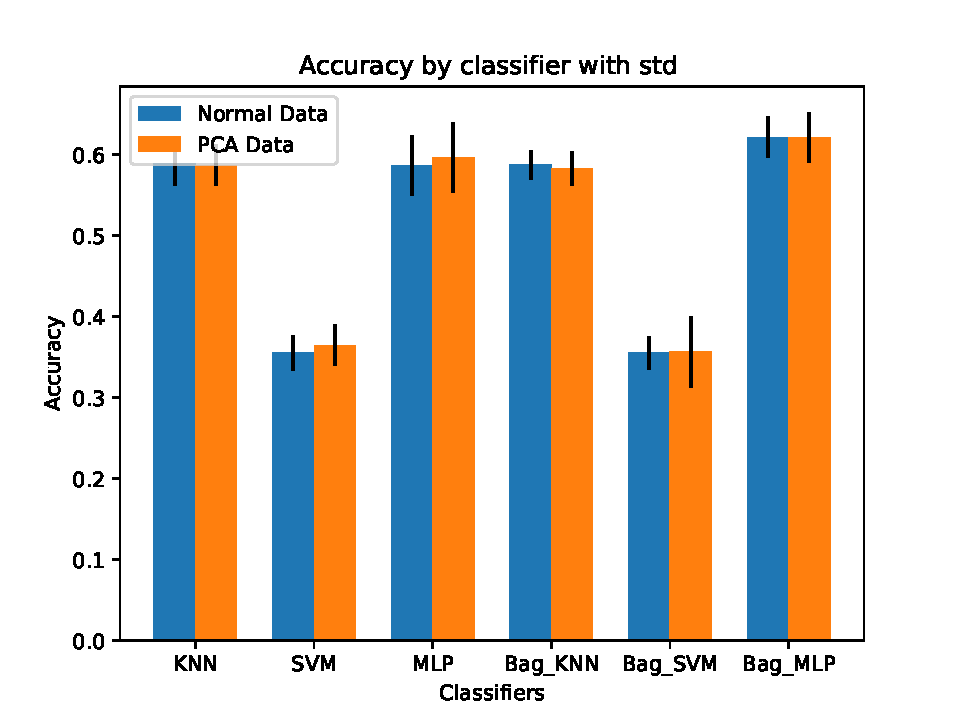
\includegraphics[scale=0.75]{graphs/GeneralAccuracy_BarPlot_ErrorBar.pdf}
    \vspace{1em}
\end{center}

It has not reached very high accuracy values in classifying music, and the reasons for this need to be investigated. These reasons may be features and train models used. However, looking at the values we have, SVM did the worst. If it is necessary to choose between KNN and MLP, MLP can be selected if the criterion is accuracy, but KNN can be chosen if the criterion is speed. Because there is no big difference in accuracy between them and MLP is a very costly operation compared to KNN.

\begin{center}
    \vspace{1em}
        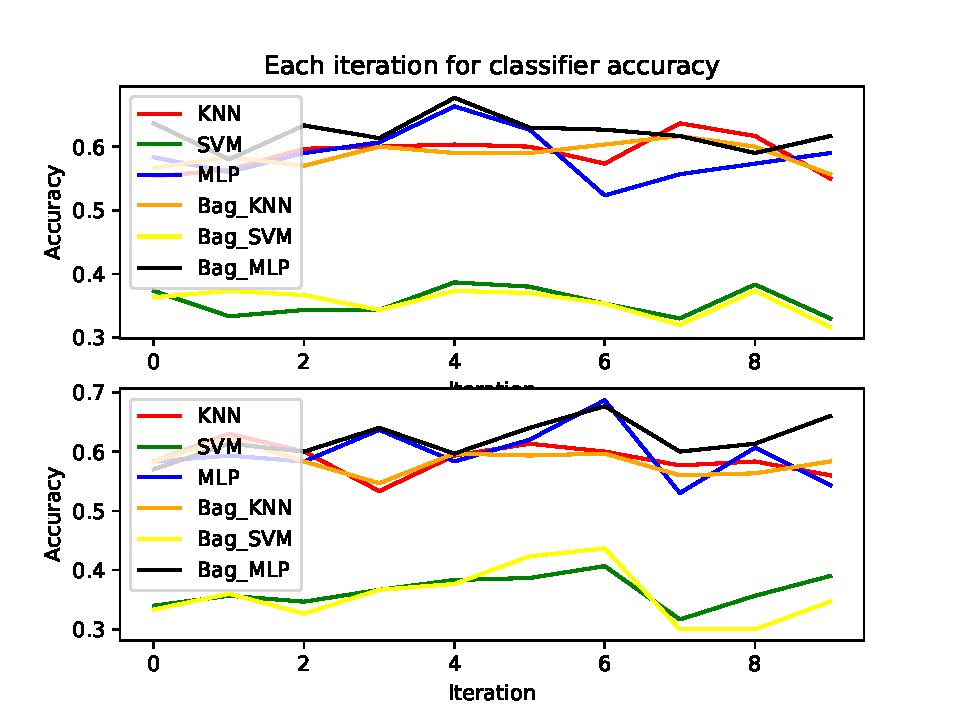
\includegraphics[scale=0.75]{graphs/Iter_by_iter.pdf}
    \vspace{1em}
\end{center}

The project had quite educational aspects for beginners like us: PreProcessing, Feature Selection and Extraction, Algorithms and their properties etc. Project has a wide range of study space and it is still improvable. 




\end{document}
